%% Mapping (chpt5)

The task of mapping was the main challenge of this work. This task consists in placing recognizable features in a map, that can later be used as landmarks by the drone to estimate its own position. The main challenge in the 3D case, is that a point needs to be observed from at least 2 different positions to be mapped. The simplest approach to map a point, is to simply triangulate its position from two different views. We will begin by exploring this approach. We will find that although this does work reasonably well when we are certain of the position of the cameras, it does not when this position is uncertain. In addition, this method does not allow to take more than two views into account. To remedy these problems we will implement a bundle adjustment step, that allows to build a map that is globally consistent. Throughout this section, we will have to make design choices to try to obtain a method that is both fast enough to work in real time, and accurate enough for the drone to control its position. To evaluate these performances, we will perform a standardized test.

\section{Structure of the map}
We will keep a keyframe-based structure for the map, but this structure will need to be adapted so that each landmark does not belong to just one keyframe. The map will contain two main data structures: a list of keyframes, and a list of landmarks. Each keyframe will contain the following information: the drone's pose estimation at the moment the keyframe was created, the estimated corrected pose of the keyframe, a list of observed keypoints, meaning their descriptor and their 2D position in the image plane of the keyframe, and for each keypoint, whether it corresponds to a landmark of the map, and which one. Each landmark will contain a descriptor and estimated 3D coordinates.\\
The map grows every time we decide to add a keyframe. When we do, the keypoints of the current image seen by the camera, along with their 2D coordinates and descriptors, are saved in a new keyframe. The descriptors are then matched with descriptors of the other keyframes, and when there is a match between two keypoints of two different keyframes, we can triangulate a new landmark into the map.\\
The main challenges are :\\
- How to triangulate new points?\\
- How to take into account when more than two keyframes see a same keypoint ?\\
- How to prevent errors from accumulating over time?\\

\section{Evaluation procedure} \label{evalproc}
All along the creation of the mapping algorithm, we will need to make design choices and to set a number of parameters. To make these decisions, we will evaluate the performance of the map using a benchmark test.
The evaluation will happen in two phases: in the map creation phase, the drone will initialize its map using four keyframes (a somewhat arbitrary number to ensure a large and enough map), and in the map testing phase, it will be moved to various known locations, and we will measure the accuracy of its position estimation. The setup used for this evaluation is illustrated on figure \ref{fig:benchmarksetup}. During the map creation phase, we will try to emulate the way the drone would initialize its map just after taking off during a real flight mission (see more in section %TODO
). First the drone is placed in a know position on a table (position A in figure \ref{fig:benchmarksetup}). There, the drone is turned on, and it begins initializing its map. The drone is then successively placed in 3 other known locations (B, then C, then D), and at each of these locations,  the drone manually receives its position. Every time this happens, the drone adds landmarks into the map, and optionally updates existing landmarks' positions, or even removes some landmarks. In reality, the drone would not know its exact position when making keyframes at points B, C, and D (position A is defined as the origin), especially at the beginning, as it would have to rely on its IMU and other internal sensors to estimate its position. To emulate this, we implement a second type of test: the robustness test, where the position that is communicated to the drone is slightly different from its real position, at each of the uncertain points (B, C, and D).\\
In the map testing phase, the drone is again placed at different known locations. This time, no information is communicated to the drone from the outside, and the drone does not modify its map. The drone estimates its position using only its camera and the map that it built during the initialization phase. We compare the drone's estimated position with its real position to evaluate the quality of the map. The two quantities we will seek to optimize are the accuracy of the drone's visual pose estimation, and the time taken to create the map.


\begin{figure}[H]
  \centering
  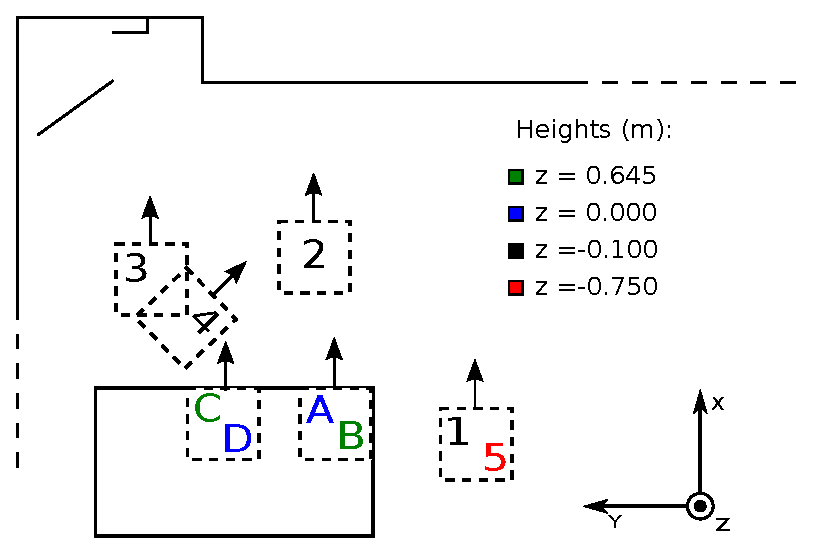
\includegraphics{benchmark_setup.eps}
  \label{fig:benchmarksetup}
  \caption{Different positions of the drone during the validation}
\end{figure}


\section{Triangulation}
Our first problem is where to put a landmark in the 3D world from two observations at two different keyframes. If all measurements were perfect, we could simply draw a ray at each keyframe that goes from the camera center and passes through the keypoint in the image plane, and those two rays would intersect at the position of the landmark. \\
Unfortunately, those lines never intersect in practice, due to various errors (measurement errors, errors in the model of the cameras, errors on the position estimation of the cameras), so we need to find a method to find the best possible location of a 3D point from the pair of images.

\subsection{Midpoint Method}
The simplest and most obvious solution is to take the midpoint of the common perpendicular of the two rays. This method is intuitive to understand geometrically, and is quite easy to compute. In practice, however its results are not very good, as there is no theoretical reason for this point to be the best.

\subsection{Linear least squares}
A more advanced method for finding the coordinates of a point from a correspondence is called Linear Least squares, and is described in Hartley & Zisserman's \textit{Multiple view geometry in computer vision} \cite{multipleviewgeometry}.
This method also has the advantage that it is already implemented in the OpenCV library.


\subsection{Optimal Correction}
If we assume that the error on observed points is random and follows a Gaussian distribution with zero mean, then the optimal solution would be to displace the pixels on both images until the resulting rays meet, keeping the displacement of the pixels as small as possible in the least squared sense. Such a solution would give the maximum likelihood estimator of the position of the 3D points, under those assumptions.
There are several algorithms in the litterature that triangulate the position of a point using optimal correction. The most popular one, proposed by Hartley and Sturm \cite{hartleysturm}, computes the solution directly but requires finding the root of a 6th degree polynomial. Kanantani et. al.'s method \cite{kanatani} finds a solution iteratively, but requires very few iterations to have an accurate solution, and in practice, is faster than the Hartley Sturm method. It also has better numerical properties, as unlike the Hartley-Sturm method, it does not have singularities at the epipoles.

\subsection{Comparison of triangulation methods}
Using the evaluation procedure described in section \ref{evalproc}, we can compare these 2 triangulation methods.

%TODO put new csv here

\begin{table}[H]
  \centering
  \caption{Comparison between triangulation methods}
  \small\addtolength{\tabcolsep}{-2pt}
  \sisetup{round-mode=places, round-precision = 3}
  \begin{tabular}{ @{} l S[table-format=2.3] S[table-format=2.3] S[table-format=2.3] S[table-format=2.3] S[table-format=2.3] @{}  }
    \toprule
    {}                 & \multicolumn{2}{c}{Accuracy} &  \multicolumn{2}{c}{Robustness} &   \multirow{2}{4em}{Computation Time (\si{\second})} \\
    {}                 & {\footnotesize Distance (\si{\meter})} & {\footnotesize Angle (\si{\radian})}
    & {\footnotesize Distance (\si{\meter})} & {\footnotesize Angle (\si{\radian})} &   \\
    \midrule
    Midpoint Method    & \num{0.121729436669}  & \num{0.052339119893} & \num{0.844616151792} & \num{0.27019708855} & \num{0.012}\\
    Optimal Correction & \num{0.0988557438948} & \num{0.0406436455673}& \num{0.775954169079} & \num{0.218538344815}& \num{0.024}\\
      \bottomrule
  \end{tabular}
  \label{fig:triangcompare}
\end{table}


The computations were timed during the accuracy test, but these timings should be the same for the robustness tests. %TODO justify this
We can see that the optimal correction method is more performant, at the cost of being computationally heavier. We will see, however, that this computation time is negligible in comparison with the time taken for bundle adjustment. Because the time difference is not significant, and because optimal correction is better motivated theoretically while also giving better results in practice, we will use the optimal correction method to triangulate points.\\
The performance increase from optimal correction is not very big however, because the biggest source of error is not gaussian noise on the measurements of the points, but errors in the position estimate of the cameras at the moment of creating the keyframes (especially in the robustness test).

\section{Bundle Adjustment}
Having a bad estimation of the keyframe's pose is problematic, as it will result in badly located landmarks, which in turn will cause a bad estimation of the camera's position when future keyframes are created. In the long term, errors will accumulate, and the map will be completely distorted. Luckily, if we have enough point correspondences between two images, it is possible to deduce the relative displacement between the two images. This means that from a set of images, we can reconstruct a scene, without even needing a prior estimation of the position of the cameras that took the images. This is good news as it means that the images can give us some absolute information about the scene, that can be used to cerrect the errors on the camera poses of the previous keyframes. The problem of adjusting camera poses and 3D point locations in order to minimize the reprojection errors of the 3D points onto the image planes is known as bundle adjustment. As stated above, bundle adjustment has the advantage of being absolute with respect to the world, and so not having errors accumulate. Another advantage of bundle adjustment, is that it can easily take into account points that are seen by more than two cameras, which is not trivial for the triangulation techniqhes described above. The main disadvantage of bundle adjustment is that it is computationally heavy, so it is important to adapt it to be useable un real time.\\
To show the advantages of bundle adjustment, we compare it with triangulation using the optimal correction method. When using bundle adjustment, optimal correction triangulation is also used to obtain an initial solution, from which we optimize.
\subsection{How it works}
%TODO

\subsection{Performance}
\begin{table}[H]
  \centering
  \caption{Performance of Bundle Adjustment}
  \small\addtolength{\tabcolsep}{-2pt}
  \sisetup{round-mode=places, round-precision = 3}
  \begin{tabular}{ @{} l S[table-format=1.3] S[table-format=1.3] S[table-format=2.3] S[table-format=1.3] S[table-format=1.3] S[table-format=2.3] @{}  }
    \toprule
    {}      & \multicolumn{3}{c}{Accuracy} &  \multicolumn{3}{c}{Robustness} \\
    {}      & {\scriptsize Distance (\si{\meter})} & {\scriptsize Angle (\si{\radian})} & {\scriptsize Time (\si{\second})}
            & {\scriptsize Distance (\si{\meter})} & {\scriptsize Angle (\si{\radian})} & {\scriptsize Time (\si{\second})} \\
    \midrule
    No Bundle Adjustment  &\num{0.0988557438948}&\num{0.0406436455673}&  {\textemdash}    &\num{0.775954169079}&\num{0.218538344815}&  {\textemdash}      \\
    With Bundle Adjustment&\num{0.0897626230568}&\num{0.029930165598} &\num{15.7027562261}&\num{1.37414105299} &\num{0.492183127143}&\num{13.8024009466}  \\
    \bottomrule
  \end{tabular}
  \label{fig:bacompare2}
\end{table}

We see that in the accuracy test, bundle adjustment gives a significant improvement to the performance of the pose estimation. In the robusteness test, however, bundle adjustment makes the results quite worse. This is surprising, as it is just in the case where the pose of the camera is uncertain that bundle adjustment should improve de result, by adjusting the pose of the camera. But because the problem is quite non linear, it is possible to fall in local minima. We will later see that by tuning the bundle adjustment phase, we can make it perform much better, and actually improve the results in the robustness test. The other big problem of bundle adjustment is the time it takes. In both tests, this time was over \SI{13}{\second}, which is a prohibitively large amount of time for real time applications. In addition to improving the performance on the robustness test, we will try to recude the time taken by the bundle adjustment.



\subsection{Tuning the Bundle Adjustment}
The main drawback of Bundle Adjustment is that it requires an iterative method to be solved and can take a lot of time, which of course is a limiting factor for a robot that builds a map in real time. Therefore it is important to optimize both the speed of the computations, and their accuracy. As is often the case, there will have to be a tradeoff between these two. To measure both the speed of the Bundle Adjustment and the accuracy of the map obtained, we will conduct some experiments using different parameters to initialize the map.

\subsubsection{Convergence of the solver}
The first element we can tune is the convergence criterion of the solver that solves the bundle adjustment problem. We will stop when the ratio of the change in the objective function to the value of this function arrives below some threshold. This ensures that the criterion scales with the problem, which is important as the size of the problem can vary during operation (as the map grows, for example). The default value of the Ceres solver is $10^{-6}$, but experimentally, we find that we can use a softer threshold to significantly speed up the computations, without impactig the quality of the results too much (and even improving them in the robustness test).

\begin{table}[H]
  \centering
  \caption{Effect of convergence criterion on Bundle Adjustment speed and performance}
  \small\addtolength{\tabcolsep}{-2pt}
  \sisetup{round-mode=places, round-precision = 3}
  \begin{tabular}{ @{} S[scientific-notation=true] S[table-format=1.3] S[table-format=1.3] S[table-format=2.3]
                                                   S[table-format=1.3] S[table-format=1.3] S[table-format=2.3] @{}  }
    \toprule
    \multirow{2}{4em}{Convergence Threshold}  & \multicolumn{3}{c}{Accuracy} &  \multicolumn{3}{c}{Robustness} \\
        & {\scriptsize Distance (\si{\meter})} & {\scriptsize Angle (\si{\radian})} & {\scriptsize Time (\si{\second})}
        & {\scriptsize Distance (\si{\meter})} & {\scriptsize Angle (\si{\radian})} & {\scriptsize Time (\si{\second})} \\
    \midrule
    \num{10}       &\num{0.0988557438948}&\num{0.0406436455673}&\num{0.528740555048}&\num{0.775553503184}&\num{0.219380944042} &\num{0.527468636632} \\
    \num{5}        &\num{0.0988557438948}&\num{0.0406436455673}&\num{0.532568186522}&\num{0.775954169079}&\num{0.218538344815} &\num{0.560289662331} \\
    \num{1}        &\num{0.0988557438948}&\num{0.0406436455673}&\num{0.536680459976}&\num{0.775954169079}&\num{0.218538344815} &\num{0.529257409275} \\
    \num{0.5}      &\num{0.0988557438948}&\num{0.0406436455673}&\num{0.532132491469}&\num{0.284057820455}&\num{0.0860006110714}&\num{0.61461224407}  \\
    \num{0.1}      &\num{0.116334787731} &\num{0.0370860746263}&\num{0.67120449245} &\num{0.244478011775}&\num{0.0982536795903}&\num{1.17620864138}  \\
    \num{0.05}     &\num{0.0684117396072}&\num{0.01622317801}  &\num{0.742543946952}&\num{0.291411483818}&\num{0.112600996782} &\num{2.11719946936}  \\
    \num{0.01}     &\num{0.0895791917611}&\num{0.032296133528} &\num{1.42051474378} &\num{0.823415005012}&\num{0.316300896325} &\num{2.77009601146}  \\
    \num{0.005}    &\num{0.0908954991063}&\num{0.0308365172421}&\num{1.53279625252} &\num{0.142093947791}&\num{0.0495629729962}&\num{4.18590991944}  \\
    \num{0.001}    &\num{0.0849543195902}&\num{0.023134969351} &\num{3.61956872419} &\num{1.034983532}   &\num{0.397193935917} &\num{4.90690393746}  \\
    \num{0.0001}   &\num{0.0842253035954}&\num{0.0258716997751}&\num{5.05812323838} &\num{1.36150222356} &\num{0.479872553731} &\num{10.4840388894}  \\
    \num{0.00001}  &\num{0.0899028376206}&\num{0.0299204957695}&\num{12.4531462789} &\num{1.4834446381}  &\num{0.528430316164} &\num{13.2059885859}  \\
    \num{0.000001} &\num{0.0897626230568}&\num{0.029930165598} &\num{15.7027562261} &\num{1.37414105299} &\num{0.492183127143} &\num{13.8024009466}  \\
    \num{0.0000001}&\num{0.0875171189566}&\num{0.0282118025117}&\num{15.7951563597} &\num{1.55886341652} &\num{0.567309620599} &\num{12.934817493}   \\
    \bottomrule
  \end{tabular}
  \label{tab:convergencetol}
\end{table}

As we can observe on table \ref{tab:convergencetol}, the more severe the convergence threshold, the better the performance on the accuracy test. On the robusteness test, however, this is true for high convergence thresholds, but when the convergence threshold is lower than \num{0.01}, the performance starts to degrade as the convergence threshold becomes lower. In both the accuracy and robustness tests, the lower the threshold, the longer it takes. We will chose a threshold of \num{0.05}, as it is a nice compromize of performance on the accuracy test, performance on the robustness test, and speed.

\subsubsection{Rejecting outliers}
When looking closer at the results of bundle adjustment, we find that a large part of the errors come from a small number of points. One possible explanation is that these points do not correspond to real world points, so that even if we have the correct position of all cameras exatly, the rays corresponding to these points will not intersect, or even be close to intersection. For this reason, after every bundle adjustment pass, we could look at the contribution of every mapped point to the objective function, and eliminate points whose error is too high. Before doing this we have to take some things into account that as a point is observed by an increasingly large number of cameras:
\begin{itemize}
  \item Its total contribution to the cost function will increase, as each observtion of a point adds a term to the objective funtion
  \item Its contribution per observation to the cost function will also increase, because every time an observation is added, the location of the point will change a bit, and its position will become less optimal if we only consider the cameras that already saw the point before.
\end{itemize}
For these reasons, we will put a different threshold on the points depending on the number of cameras that see the point. If a point is seen by a large number of cameras, we will allow it to have larger errors in the objective function before removing it.











\section{Map Initialization}
A robot needs a map lo localize itself within it, but it needs to know its position to find the postion of surrounding objects and build a map. Because the mapping and localization tasks are mutually dependent on one another, there needs to be a special procedure to build a map from nothing when it does not exist yet. Arbitrarily, we decide that the position of the drone when it starts flying is the origin (in all 6 degrees of freedom) of the map. However, with only a monocular camera, it is not possible to find the exact location of any visual features from one observation only, views from at least two different positions are needed to triangulate points.


%%blabla

To reach the position from which the drone will take a second view and triangulate points, the drone has to fly blindly. Blindly here means without using a map la localize itself visually, but the drone can still use its other sensors (IMU and ultrasonic sensor) to obtain an estimate of its postion. Because the ultrasonic sensor is much more accurate than the IMU, and gives an absolute measure, we will mostly rely on this sensor to estimate the relative position from where we take the second view. Because the ultrasonic sensor only gives the distance from the bottom of the drone to the ground, the drone should fly straight up from its first position (the origin) to reach its second position.\\
Once in its second position, the drone can match seen keypoints from both views, and from its estimated position, triangulate those points to the map. However, the drone's estimation of its pose is prone to errors, especially as it only used its ultrasonic sensor and IMU. There errors can be corrected with the information from the cameras, because of we have %TODO how many
matching observations, we can compute the fundamental matrix, and know exactly the displacement between the two views. Refining the poses of the views and the location of the landmarks simultaneously such as to minimize the reprojection error is a nonlinear optimization problem known as Bundle Adjustment. Using Bundle adjustment, we can refine the position of the second view, and use the ultrasonic sensor information to fix the scale. Another advantage of Bundle Adjustment is that it allows to take into account more than 2 views of a point.
